
% this file is called up by thesis.tex
% content in this file will be fed into the main document

%: ----------------------- introduction file header -----------------------
\chapter{Background} \label{cha:background}

% the code below specifies where the figures are stored
\ifpdf
    \graphicspath{{2_background/figures/PNG/}{2_background/figures/PDF/}{2_background/figures/}}
\else
    \graphicspath{{2_background/figures/EPS/}{2_background/figures/}}
\fi

% ----------------------------------------------------------------------
%: ------------------------------- content ----------------------------- 
% ----------------------------------------------------------------------

The main contributions of this thesis are methods for the automatic generation of
user-customizable media galleries for the visual and audial summarization of events.
To provide context for the approaches proposed in the later parts of the thesis,
we start with an introduction of related background technologies.
The current \autoref{cha:background} covers the Semantic Web, Linked Data,
and the Resource Description Framework (RDF).
The following \autoref{cha:social-networks} will cover social networks
by first providing a~definition and classification of social networks,
and then introducing popular social networks and some of their core features.

\section{Semantic Web}
The lexical database WordNet~\cite{Fellbaum1998} by the Cognitive Science Laboratory
of Princeton University defines\footnote{\url{http://wordnetweb.princeton.edu/perl/webwn?s=semantic}}
the term \emph{semantic} as \emph{of or relating to meaning or the study of meaning}.
The same source defines\footnote{\url{http://wordnetweb.princeton.edu/perl/webwn?s=world+wide+web}}
the term \emph{Web}, which is a~common form for the complete term \emph{World Wide Web} (or just \emph{WWW}) as
\emph{computer network consisting of a~collection of internet sites that offer text and graphics and
sound and animation resources through the hypertext transfer protocol}.
Finally WordNet defines\footnote{\url{http://wordnetweb.princeton.edu/perl/webwn?s=meaning}}
the term \emph{meaning} as \emph{the message that is intended or expressed or signified}, or
\emph{the idea that is intended}.

The combined term \emph{Semantic Web} has been coined by Sir Tim Berners-Lee,
the inventor of the World Wide Web and Director of the World Wide Web Consortium,
in a~May 2001 article co-published with James Hendler and Ora Lassila
in the Scientific American~\cite{BernersLee2001}.
Therein, the authors write: 

\begin{quotation}
``The Semantic Web will bring structure to the meaningful content of Web pages,
creating an environment where software agents roaming from page to page
can readily carry out sophisticated tasks for users. [\ldots]
The Semantic Web is not a~separate Web but an extension of the current one,
in which information is given well-defined meaning, better enabling computers and people
to work in cooperation.
The first steps in weaving the Semantic Web into the structure of the existing Web
are already under way.
In the near future, these developments will usher in significant new functionality
as machines become much better able to process and \emph{understand} the data
that they merely display at present.''
\end{quotation}

We are currently experiencing a~fundamental shift from the World Wide Web (WWW) to the Semantic Web,
a~shift from moving bits to moving bits with a~meaning.
This can have a~huge impact, which might not be as drastic as Tim Berners-Lee describes
in his Scientific American article, but which might introduce many small improvements,
like more accurate search results, or more intelligent price comparison services etc.
\autoref{fig:fundamental-shift} illustrates this idea.

\begin{figure}[htbp!]
\begin{center}
  \subfloat[Bits without meaning.]{\label{fig:fundamental-shift-1}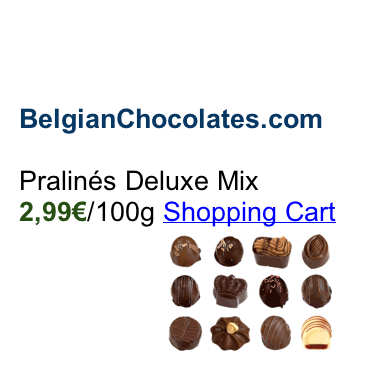
\includegraphics[width=0.3\textwidth]{fundamental-shift-1.png}}                
  \subfloat[Bits with a~meaning.]{\label{fig:fundamental-shift-2}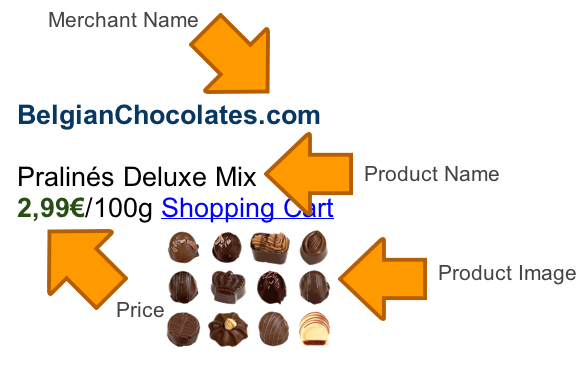
\includegraphics[width=0.468\textwidth]{fundamental-shift-2.png}}
  \caption{Fundamental shift from moving bits to moving bits with a~meaning.}
  \label{fig:fundamental-shift}  
\end{center}    
\end{figure}

\subsection{The Non-Semantic Web} \label{sec:non-semantic-web}
To differentiate the Semantic Web from the non-semantic Web, it helps to step back one step and
see why the non-semantic Web is not semantic.
The Web is a~system of interlinked hypertext documents accessed through the Internet.
These documents are typically marked up in HTML, a~language that defines a~syntax
understandable to user agents like Web browsers, however,
not one that provides meaning beyond the level of text layout.
This means that an HTML snippet like
\begin{verbatim}
<h1>The Catcher in the Rye</h1>
<h2>J. D. Salinger</h2>
\end{verbatim}
reveals that \emph{The Catcher in the Rye} is a~level one header element and
that \emph{J. D. Salinger} a~level two header element,
but to a~machine it is not evident that the prior is the title of a~book,
and that the latter is (i), an author, and (ii), the author of \emph{The Catcher in the Rye}.

\subsection{Structured Data on the Web}
A very first step to add semantics to the Web is using tabular data.
\autoref{tab:sample-table-structured-data} shows an example for such tabular data.
To human beings (interested in sports), the meaning of the columns is clear:

\begin{table}[b]
 \begin{center}
  \begin{tabular}{l*{6}{c}r}
Team              & P & W & D & L & F  & A & Pts \\
\hline
Manchester United & 6 & 4 & 0 & 2 & 10 & 5 & 12  \\
Celtic            & 6 & 3 & 0 & 3 &  8 & 9 &  9  \\
Benfica           & 6 & 2 & 1 & 3 &  7 & 8 &  7  \\
FC Copenhagen     & 6 & 2 & 1 & 2 &  5 & 8 &  7  \\
  \end{tabular}
\caption{Sample table with structured data for sports results.}
\label{tab:sample-table-structured-data}
 \end{center}
\end{table}

\begin{itemize}
\item P = matches \textbf{P}layed
\item W = \textbf{W}on 
\item D = \textbf{D}rew
\item L = \textbf{L}oss
\item F = Goals \textbf{F}or
\item A = Goals \textbf{A}gainst
\item Pts = \textbf{P}oin\textbf{ts}
\end{itemize}

The problem, however, is for machines to understand the structure of the table.
Let us imagine one wanted to automate the task of retrieving sports results.
While it is a~relatively straightforward job to implement a~scraper bot that
searches for column titles like ``P'', ``W'', ``D'' etc.,
it would require the same work over and over again for different languages
(for example German for: ``Sp.'', ``g.'', ``u.'', ``v.'', ``Tore'', ``Pkte.'').
The German-speaking reader might have noticed that the exemplary German system listed here
does not differentiate between \emph{goals for} and \emph{goals against}, but only has a~list of \emph{Goals}.
Tiny differences like this make the scraping approach so brittle.
If data providers were to use unique column identifiers like URIs, the problem would be mostly gone.
In the concrete example, rather than using ``D'' or ``u.'', which both mean that the result was a~tie,
the machine-readable column name could be identified by the URI
\url{http://dbpedia.org/page/Tie_%28draw%29}.
In the next Section we therefore introduce the structured knowledge base DBpedia.

\subsection{The Structured Knowledge Base DBpedia}
An often reoccurring (however not binding) pattern in the Semantic Web world
is the use of DBpedia~\cite{Auer2007} URIs as a~hub for identifying concepts by URIs.
DBpedia is a~Semantic Web knowledge base with the objective of
automatically extracting structured data from the human-generated information from
the online encyclopedia Wikipedia~\footnote{\url{http://en.wikipedia.org/wiki/Main_Page}}.
This structured information is then made available on the World Wide Web in many variations,
for example as JSON~\cite{Crockford2006}, HTML~\cite{LeHors1999}, XML~\cite{Bray1998},
and many RDF~\cite{Klyne2004} serializations.
DBpedia allows for querying relationships and properties associated with Wikipedia resources,
including links to other related datasets.
As outlined before, the concept of a~tie draw in the sense of sports
could thus be uniquely identified by the DBpedia URI \url{http://dbpedia.org/page/Tie_%28draw%29},
free of all ambiguity.
Similar knowledge bases are among others Freebase~\cite{Markoff2007},
YAGO~\cite{Suchanek2007}, or Cyc~\cite{Wilkins1997}.

\subsection{Semantics in HTML Version 4 and 5}
As outlined in \autoref{sec:non-semantic-web}, HTML versions 4~\cite{LeHors1999} and 5~\cite{Hickson2011}
contain a~basic level of semantics.
The main focus, however, is on the separation of semantics from presentation.
For example the \texttt{<b>} and the \texttt{<strong>} tags both have the same visual effect:
they make the node value appear in a~bold face \textbf{like so}.
Visually, there is no way to differentiate between the two, however,
semantically the difference exists and is well-defined:
\texttt{<strong>} should be used when one wants to give special emphasis on something,
screenreaders will typically read out such text with a~more emphasized voice.
In contrast \texttt{<b>} should be used if only visually one wants to create a~bold face look.
In the following, we present a~list of semantic HTML tags and attributes and their meaning.
The list is inspired by an
extension\footnote{\url{https://addons.mozilla.org/en-us/firefox/addon/semantic-checker/}}
for the Web browser Firefox.

\paragraph{Semantic HTML4 Elements}
\begin{itemize}
\item \texttt{abbr} specifies an abbreviation, \texttt{acronym} specifies an acronym.
\item \texttt{h1-h6} specify level 1-6 headers, \texttt{caption} specifies a~caption for a~table.
\item \texttt{blockquote} specifies a~block-level quotation
(a source in form of a~URI may be specified via the \texttt{@cite} attribute),
\texttt{cite} specifies a~citation.
\item \texttt{dl} specifies a~definition list, \texttt{dt} specifies a~definition term in a~definition list,
\texttt{dd} specifies the definition of a~term in a~definition list.
\item \texttt{em} specifies an emphasis, \texttt{strong} specifies a~strong emphasis.
\item \texttt{code} specifies a~code snippet, \texttt{dfn} specifies an inline definition of a~single term,
\texttt{address} specifies contact information for the document author,
\texttt{legend} specifies a~legend for \texttt{fieldset} containers for adding structure to forms,
\texttt{samp} specifies sample output from a~script or program.
\end{itemize}

\paragraph{Semantic HTML5 Elements}
\begin{itemize}
\item \texttt{article} specifies an independent item section of content,
\texttt{aside} specifies a~section of a~page that consists of content that is tangentially related
to the content around the \texttt{aside} element, and which could be considered separate from that content,
\texttt{header} specifies a~group of introductory or navigational aids,
\texttt{footer} specifies a~footer for its nearest ancestor sectioning content or sectioning root element,
\texttt{nav} specifies a~section with navigation links.
\item \texttt{figure} specifies some flow content,
\texttt{mark} specifies a~run of text in one document marked or highlighted for reference purposes
due to its relevance in another context, \texttt{meter} specifies a~scalar measurement within
a~known range, or a~fractional value.
\item \texttt{audio} specifies a~sound or an audio stream, \texttt{video} specifies a~video or movie.
\item \texttt{progress} specifies the completion progress of a~task,
\texttt{time} specifies either a~time on a~24 hour clock,
or a~precise date in the calendar (optionally with a~time and a~time-zone offset),
\texttt{command} specifies a~command that the user can invoke.
\item \texttt{details} specifies a~disclosure widget
from which the user can obtain additional information or controls,
\texttt{datalist} specifies the list that represent predefined options for input elements.
\item \texttt{keygen} specifies a~key pair generator control,
\texttt{output} specifies the result of a~calculation,
\texttt{ruby} allows one or more spans of phrasing content to be marked with ruby annotations.
\end{itemize}

\paragraph{HTML5 Input Attributes}
\begin{itemize}
\item \texttt{datetime} specifies a~control for setting the element's value
to a~string representing a~global date and time (with timezone information).
\item \texttt{datetime-local} specifies a~control for setting the element's value
to a~string representing a~local date and time (with no timezone information).
\item \texttt{date} specifies a~control for setting the element's value
to a~string representing a~date, \texttt{month} specifies a~control
for setting the element's value to a~string
representing a~month, \texttt{week} specifies a~control for setting the element's value
to a~string representing a~week.
\item \texttt{time} specifies a~control for setting the element's value
to a~string representing a~time (with no timezone information.
\item \texttt{number} specifies a~control for setting the element's value
to a~string representing a~number.
\item \texttt{range}  represents an imprecise control for setting the element's value
to a~string representing a~number.
\item \texttt{email} specifies a~control for editing a~list of email addresses
given in the element's value.
\item \texttt{url} specifies a~control for editing an absolute URL
given in the element's value.
\item \texttt{search} specifies a~one-line plain-text edit control
for entering one or more search terms.
\item \texttt{color} specifies a~color-well control for setting the element's value
to a~string representing a~simple color.
\end{itemize}

\section{Resource Description Framework}

\section{Linked Data}
Linked Data~\cite{BernersLee2006} defines a~set of agreed-on best practices and
principles for interconnecting and publishing structured data on the Web.
It uses Web technologies like HTTP~\cite{Fielding1999} and URIs~\cite{BernersLee2005}
to create typed links between different sources.
The portal LinkedData.org defines Linked Data as being
\textit{``about using the Web to connect related data that wasn't previously linked,
or using the Web to lower the barriers to linking data currently linked using other methods''}. 

\subsection{The Linked Data Principles}
Tim Berners-Lee defines the four rules for Linked Data in a~W3C Design Issue~\cite{BernersLee2006} as follows:
\begin{enumerate}
\item Use URIs as names for things.
\item Use HTTP URIs so that people can look up those names.
\item When someone looks up a~URI, provide useful information, using the standards (RDF*, SPARQL).
\item Include links to other URIs, so that they can discover more things.
\end{enumerate}

Linked Data uses RDF~\cite{Klyne2004} to create typed links between things in the world,
the result is oftentimes referred to as the Web of Data.
As outlined before, RDF encodes statements about things in the form of
subject, predicate, object triples.
If subject and object have URIs from different namespaces,
Bizer \emph{et al.} speak of \emph{RDF links} in~\cite{Bizer2007}.
An examplary RDF link taken from~\cite{Bizer2009} stating that a~description of the movie Pulp Fiction
from the Linked Movie Database~\cite{Hassanzadeh2009} and from DBpedia are in fact talking about the same movie
can be seen in \autoref{code:rdflink}.

\begin{lstlisting}[caption={[Exemplary RDF link.]{Exemplary RDF link stating that a~description of the movie Pulp Fiction from the Linked Movie Database~\cite{Hassanzadeh2009} and from DBpedia are in fact talking about the same movie.}},label={code:rdflink}]
http://data.linkedmdb.org/resource/film/77
http://www.w3.org/2002/07/owl\#sameAs
http://dbpedia.org/resource/Pulp_Fiction_%28film%29
\end{lstlisting}

\subsubsection{The Linked Open Data Cloud}\label{sec:lodcloud}
The Linking Open Data (LOD) project~\cite{Bizer2011} is the most visible Linked Data effort.
The project's objective is to identify existing datasets with open licenses,
convert them to RDF whilst obeying the Linked Data principles, and finally publish them on the Web.
Due to its open structure everyone can contribute to the project by publishing a~dataset and
interlinking it to existing datasets.
Today, the project includes datasets of big names such as the BBC, Thomson Reuters,
or the Library of Congress to name just a~few.
The current state of the Linking Open Data project can be seen in the so-called Linked Open Data cloud,
a~diagram that depicts the interconnectedness of each dataset.
The state of the LOD cloud as of September 2010 can be seen in \autoref{fig:lod-cloud}.

\begin{figure}[htbp!]
\begin{center}
  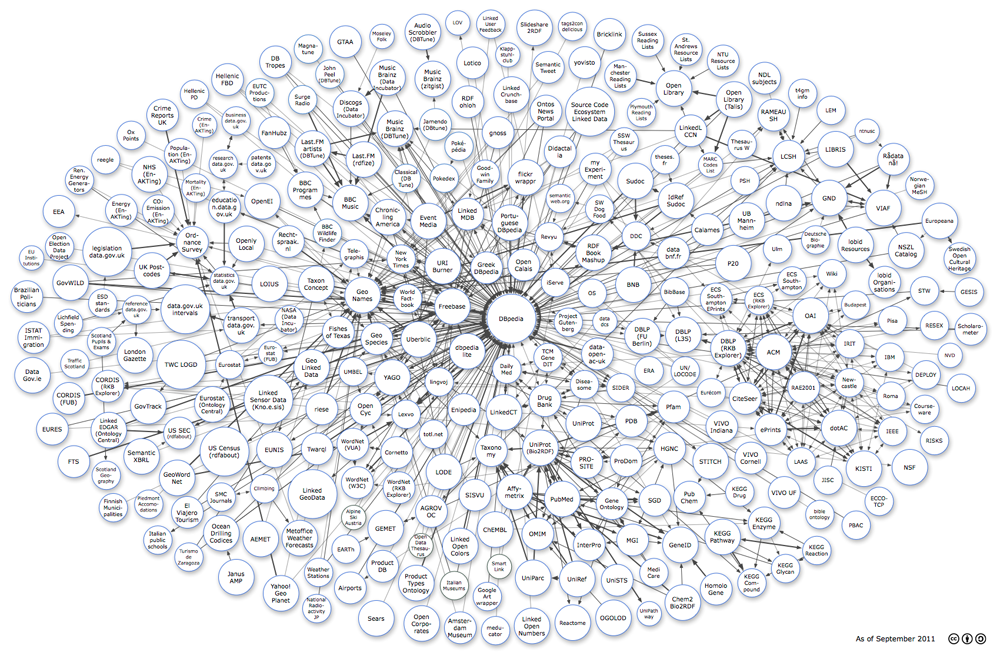
\includegraphics[width=1.0\textwidth]{lod-cloud.png}    
  \caption[The Linked Open Data cloud as of September 2010.]{The Linked Open Data cloud as of September 2010, by Richard Cyganiak and Anja Jentzsch. Source: \url{http://lod-cloud.net/}}    
  \label{fig:lod-cloud}
  \end{center}  
\end{figure}

\section{Conclusion}